

\subsubsection{Figure-Eight Map and Distance Mapping}
\label{Figure-eight track}
The control strategies are evaluated in CARLA, in which a custom map is used, which is generated using Roadrunner. The evaluation is performed on a closed loop figure-eight, illustrated in figure~\ref{fig:figure8_combined}. The figure-eight ensures vehicles arrive at the intersection continuously and is generated using parametric equations, best described by equation~\ref{MAP}
\begin{equation}
\label{MAP}
    x(t) = -R\sin{t}, \ y(t) = -R\sin{2t}, \ t\in[0,2\pi],
\end{equation}
with radius \(R \)(m), and the position \(t\)(rad). The negative sign guarantees that the standard drive direction of AVs in CARLA is aligned with increasing values of \(t\). 
This parametric setup, results in a closed loop track with two loops of identical size, which intersect exactly in the middle at \(t = \pi\), which is the location of the intersection and also the point of conflict, which both barrier and FAS controller manage. Vehicles traverse this intersection from two sides, either at respectively \(t=\pi\) or \(t=0\) (equivalently \(t=2\pi\)). 
\begin{figure}[H]
    \centering
    % First Subfigure (Left)
    \begin{subfigure}[b]{0.48\linewidth}
        \centering
        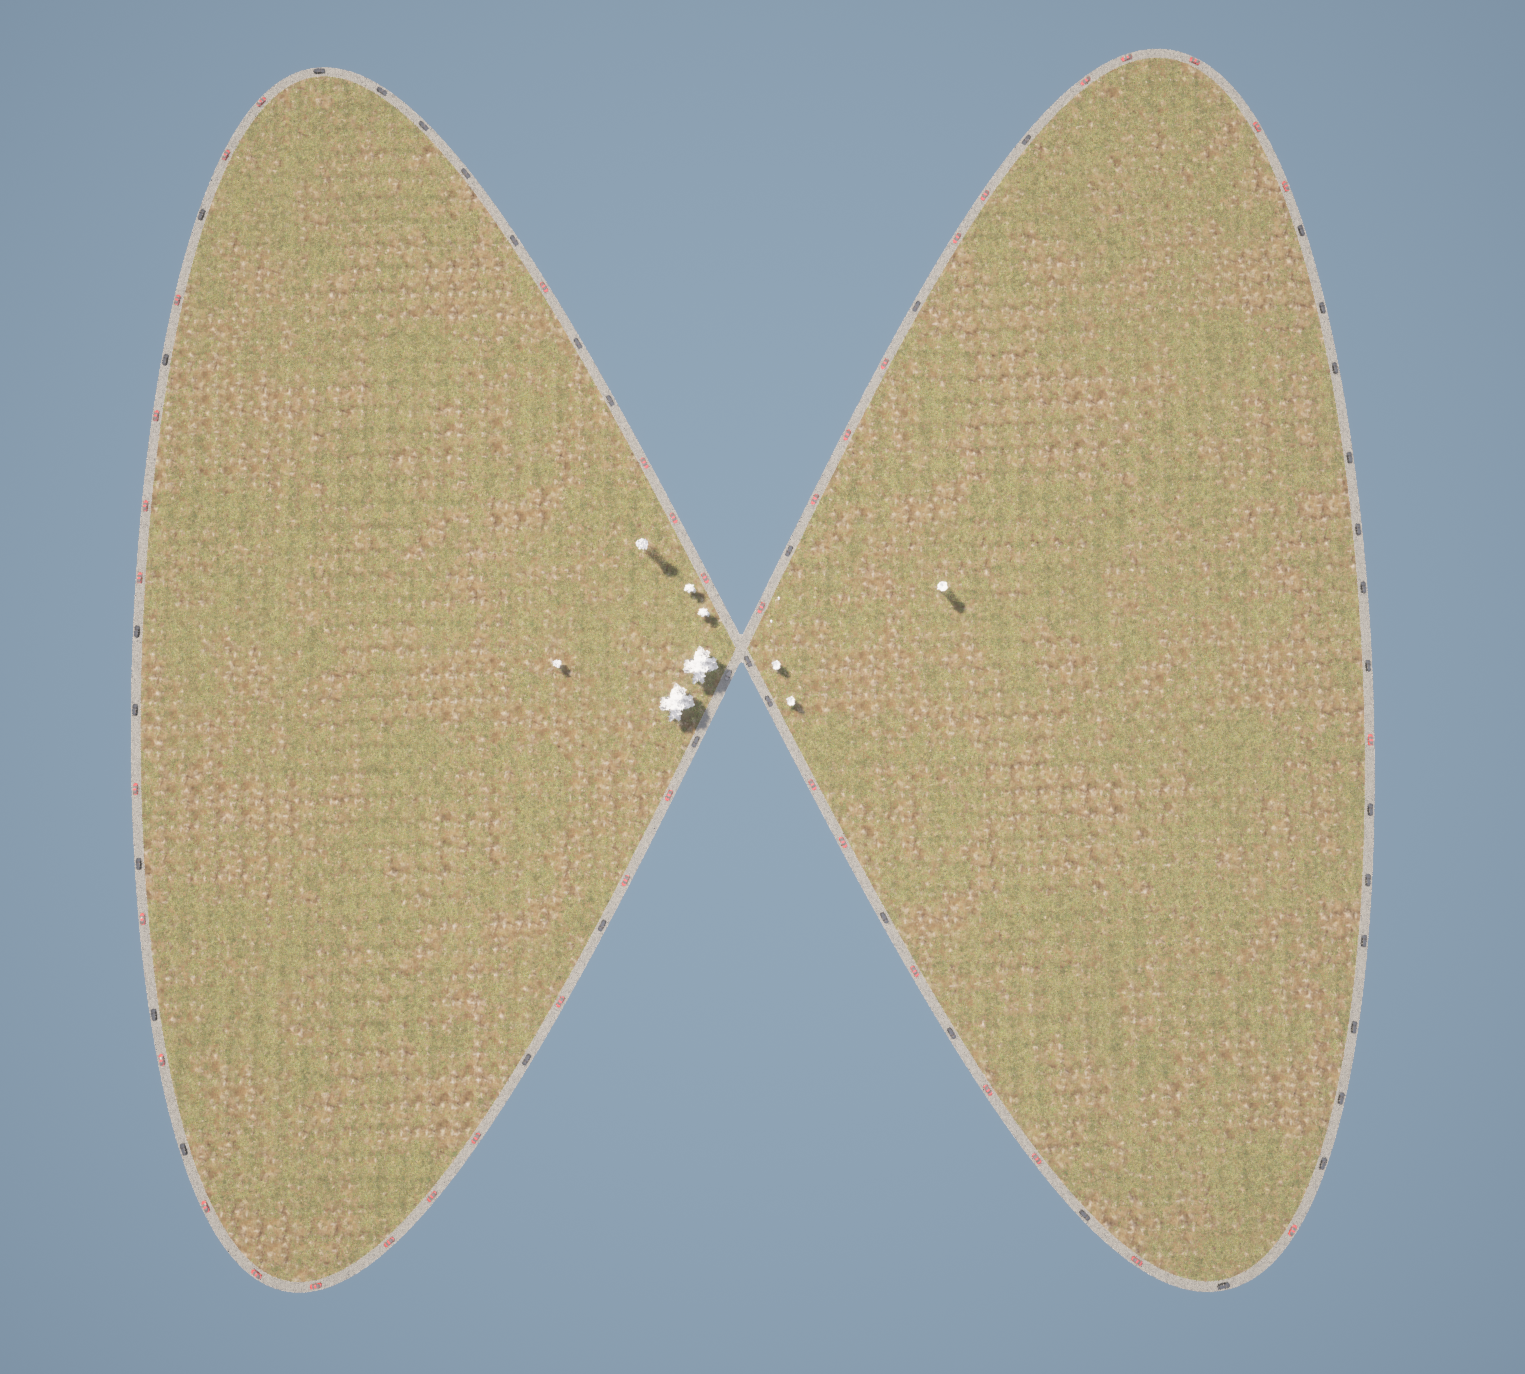
\includegraphics[width=\linewidth]{Screenshot from 2026-06-17 16-37-56.png}
        \caption{Overview of complete figure-eight}
        \label{fig:figure8_main}
    \end{subfigure}
    \hfill % Pushes the second subfigure to the right edge
    % Second Subfigure (Right)
    \begin{subfigure}[b]{0.48\linewidth}
        \centering
        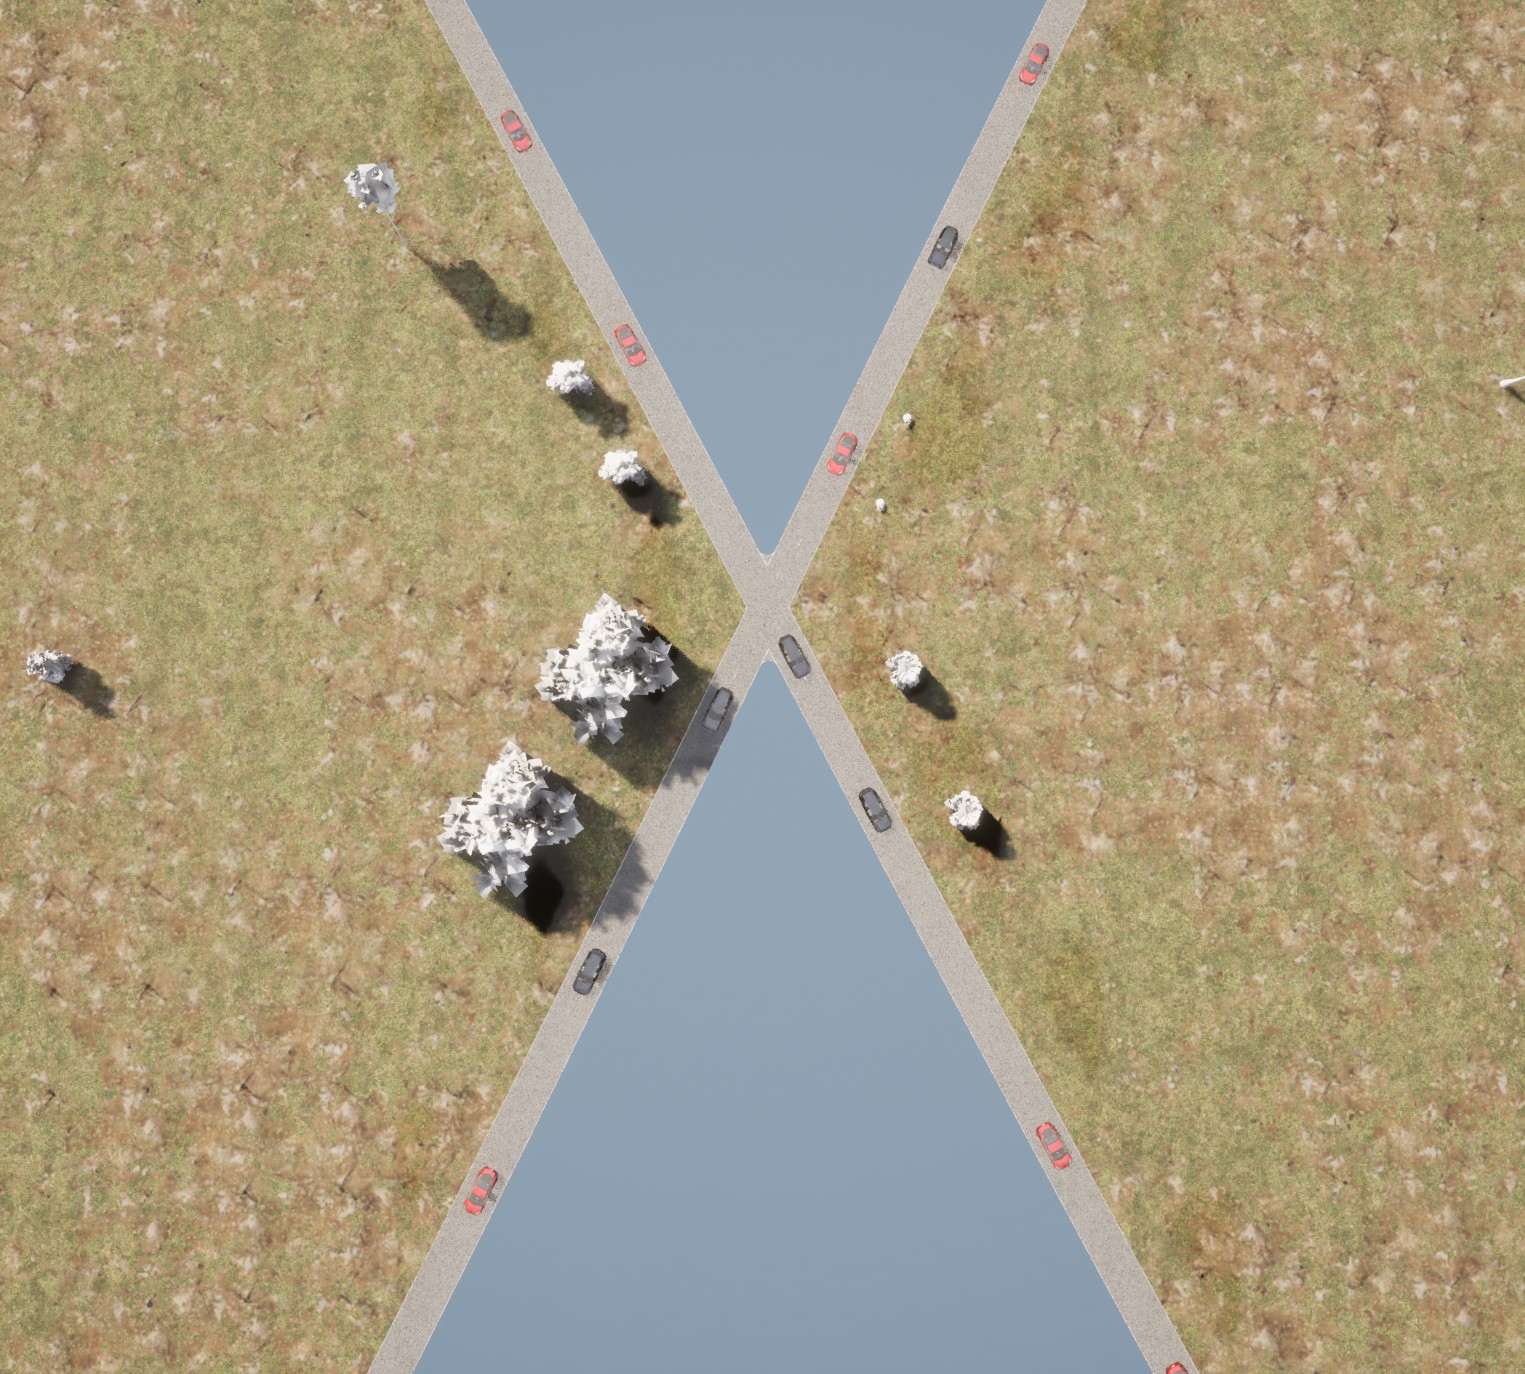
\includegraphics[width=\linewidth]{Screenshot from 2026-06-17 16-38-17.png}
        \caption{Figure-eight zoomed in at intersection}
        \label{fig:figure8_zoom}
    \end{subfigure}
    
    % Main Caption for the entire figure block
    \caption{Figure-eight Map: showing the complete map and a detailed close-up of the intersection with vehicles showing in red and black.}
    \label{fig:figure8_combined}
\end{figure}

On the figure-eight track, the position of an AV, is described by the parametric coordinate \(t\). However, the parametric coordinate is not suitable for the control strategies used in both simulations, since a difference between values of \(t\)  responds to the driven Euclidean distance. Nevertheless, the actual distance driven on the track is Geodesic. To resolve this issue, a distance mapper is used. At initialization, the distance mapper calculates the Arc Length \(L\)(m) using equation~\ref{arc length}
\begin{equation}
\label{arc length}
L =
\int_0^{2\pi}
\sqrt{
\left(\frac{dx}{dt}\right)^2 +
\left(\frac{dy}{dt}\right)^2
}
\,dt,
\end{equation} which is evaluated between 100000 equally spaced values of \(t\). The resolution of 100000 gives an accurate approximation of the true Geodesic distance by calculating the Euclidean distance of the small segments. The small segments are summed, and stored in a lookup table where each value of \(t\) corresponds to a geodesic distance \(s\)(m). Throughout the remainder of this chapter, linear interpolation is used to map from distance \(s\) to \(t\), section~\ref{Vehicle Fleet},  and from \(t\) to \(s\), section~\ref{Headway Control}.
